%-------------------------------------------------------%
\section{概要} \label{sec:tutorial_real_intro}
%-------------------------------------------------------%
本章では、以下の流れ(図\ref{fig:howto}も参照)に従う簡単な場合を例にして、
現実大気実験の基本的な実行手順を示す。
\begin{enumerate}
\item  入力データの準備(入力データは各自で準備しなければならない)
\item  \texttt{pp}      : 地形データの作成
\item  \texttt{init}    : 初期値・境界値データの作成
\item  \texttt{run}     : シミュレーションの実行
\item  \texttt{sno}     : 出力データを\grads で読み込み可能な\netcdf 形式に変換(オプション)
\end{enumerate}

\begin{figure}[b]
\begin{center}
  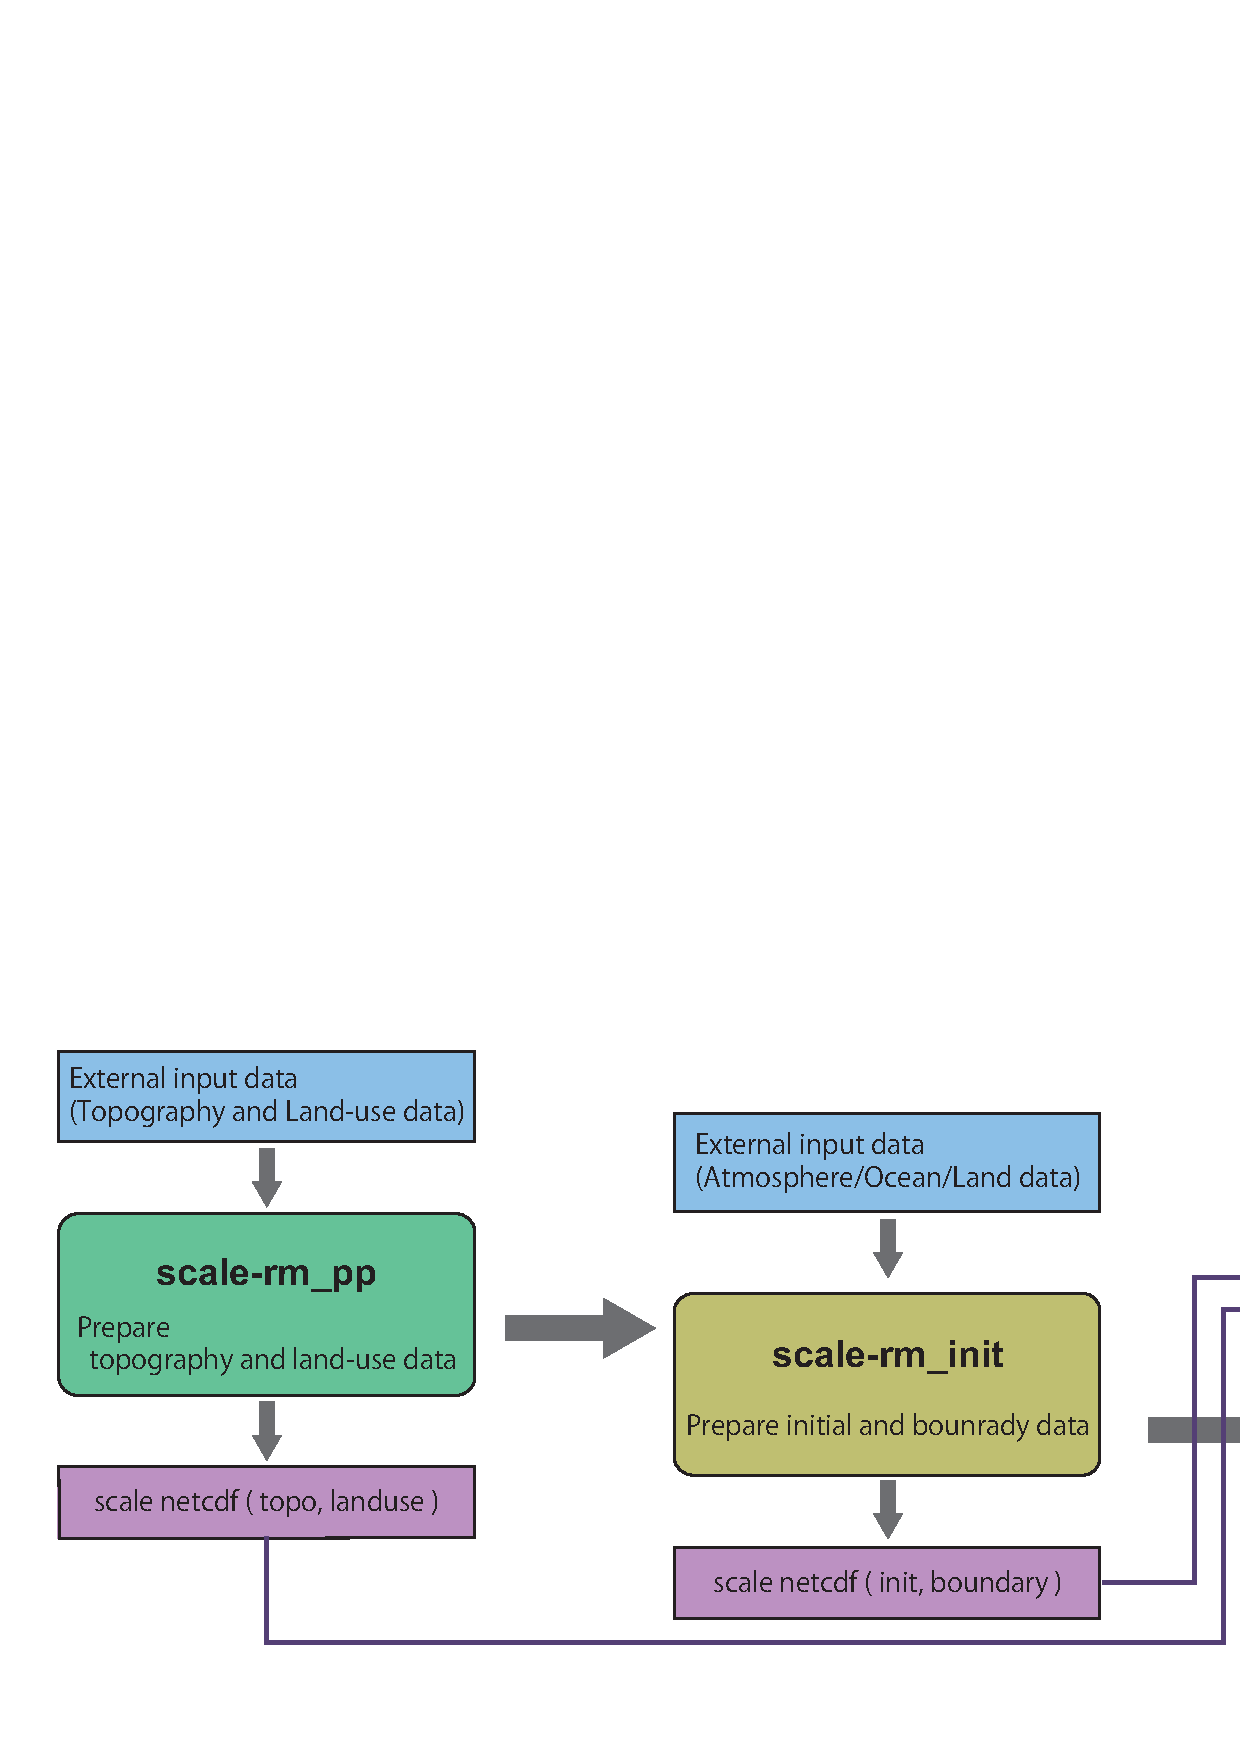
\includegraphics[width=0.9\hsize]{./../../figure/real_procedure.pdf}\\
  \caption{\scalerm におけるモデルの実行手順}
  \label{fig:howto}
\end{center}
\end{figure}

これ以降の説明では、\texttt{scale-{\version}/scale-rm/test/tutorial/}の絶対パスを
\verb|${Tutorial_DIR}|と書くことにする。

本章のチュートリアルで用いる計算領域の設定を表\ref{tab:grids}に示す。
また、対象とする計算領域を図\ref{fig:tutorial_real_domain}に示す。
本チュートリアルの目的は、\scalerm を用いて現実大気実験を実施する方法を短時間で学ぶことである。
そのために、計算が短時間で終わるように実験を設定している。
したがって、この設定が物理的に妥当な実験として適切とは限らないことに注意が必要である。
実際の研究を行うときには、必要に応じて実験設定を検討すべきである。

\begin{table}[h]
\begin{center}
  \caption{実験設定の概略}
  \label{tab:grids}
  \begin{tabularx}{150mm}{|l|X|} \hline
    \rowcolor[gray]{0.9} 項目 & 設定 \\ \hline
    MPIプロセス分割 (東西 x 南北) & 2 x 2 (合計4プロセス) \\ \hline
    水平格子数 (東西 x 南北) & 90 x 90 \\ \hline
    鉛直層数                 & 36 層                  \\ \hline
    水平格子間隔             & $\Delta x = \Delta y =$ 20 km       \\ \hline
    積分期間 & 2007年7月14日 18UTC $\sim$ 15日00UTC (6時間積分) \\ \hline
    時間ステップ間隔 & 90 sec (全 240 steps) \\ \hline
  \end{tabularx}
\end{center}
\end{table}

\begin{figure}[tb]
\begin{center}
  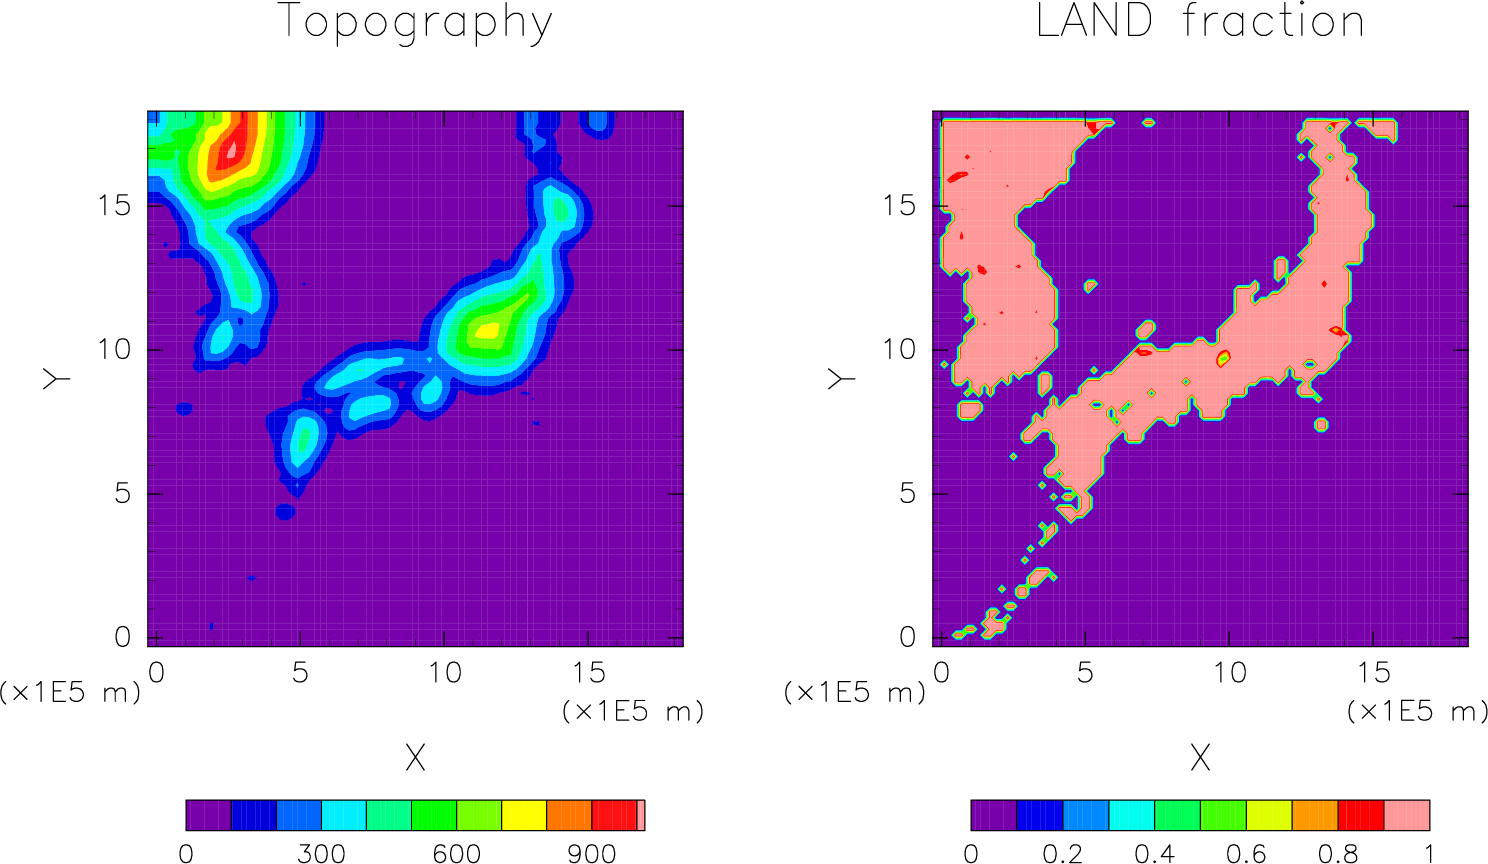
\includegraphics[width=1.0\hsize]{./../../figure/real_domain.pdf}\\
  \caption{計算領域の地形と海陸分布。}
  \label{fig:tutorial_real_domain}
\end{center}
\end{figure}
